\documentclass{article}

\usepackage{graphicx}
\usepackage{subcaption}
\usepackage{pgffor}
\usepackage{amsmath, amsthm, amssymb, amsfonts}
\usepackage{thmtools}
\usepackage{graphicx}
\usepackage{setspace}
\usepackage{geometry}
\usepackage{float}
\usepackage{hyperref}
\usepackage[utf8]{inputenc}
\usepackage[english]{babel}
\usepackage{framed}
\usepackage[dvipsnames]{xcolor}
\usepackage{tcolorbox}

\colorlet{LightGray}{White!90!Periwinkle}
\colorlet{LightOrange}{Orange!15}
\colorlet{LightGreen}{Green!15}

\newcommand{\HRule}[1]{\rule{\linewidth}{#1}}

\declaretheoremstyle[name=Theorem,]{thmsty}
\declaretheorem[style=thmsty,numberwithin=section]{theorem}
\tcolorboxenvironment{theorem}{colback=LightGray}

\declaretheoremstyle[name=Proposition,]{prosty}
\declaretheorem[style=prosty,numberlike=theorem]{proposition}
\tcolorboxenvironment{proposition}{colback=LightOrange}

\declaretheoremstyle[name=Principle,]{prcpsty}
\declaretheorem[style=prcpsty,numberlike=theorem]{principle}
\tcolorboxenvironment{principle}{colback=LightGreen}

\setstretch{1.2}
\geometry{
    textheight=9in,
    textwidth=5.5in,
    top=1in,
    headheight=12pt,
    headsep=25pt,
    footskip=30pt
}

% ------------------------------------------------------------------------------

\begin{document}

% ------------------------------------------------------------------------------
% Cover Page and ToC
% ------------------------------------------------------------------------------

\title{ \normalsize \textsc{}
		\\ [2.0cm]
		\HRule{1.5pt} \\
		\LARGE \textbf{\uppercase{CS 460: INTRO TO COMPUTATIONAL ROBOTICS}
		\HRule{2.0pt} \\ [0.6cm] \LARGE{Assignment 3} \vspace*{10\baselineskip}}
		}
\date{}
\author{\textbf{Lorenzo Nieto} \\ len44@rutgers.edu \\
    \textbf{Tasha Pais} \\ tdp74@rutgers.edu \\
		Rutgers University, Department of Computer Science \\
		December 13, 2023}


\maketitle
\newpage

\section{Setup maps and generate controls}
\subsection{Generate 4 maps with landmarks}
The file "map\textunderscore generator.py" handles map generation. It receives arguments --landmarks k and --name path. It generates a map with k landmarks with x and y coordinates each uniformly sampled in the range [0, 2] and saves the landmarks map in the file specified by path.
\subsection{Generate robot control sequences}
Running the file "controls.py" will populate the "controls" folder with two control files for each landmark map, making a total of ten control files. To generate a sequence of controls, first a start configuration was randomly generated. It was ensured that the initial configuration would stay 0.2m from the boundary. Then, a random control within the robot's limits was generated and integrated forward for two seconds. Only controls with positive velocity were generated to give the robot a smoother trajectory and make visualization easier. At each integration step, it was ensured that the robot stayed within 0.2m from the boundary and if it didn't, a new control was generated. Ten controls were generated in this way for each control file. Finally, a plot showing the trajectories of all the control files was generated.
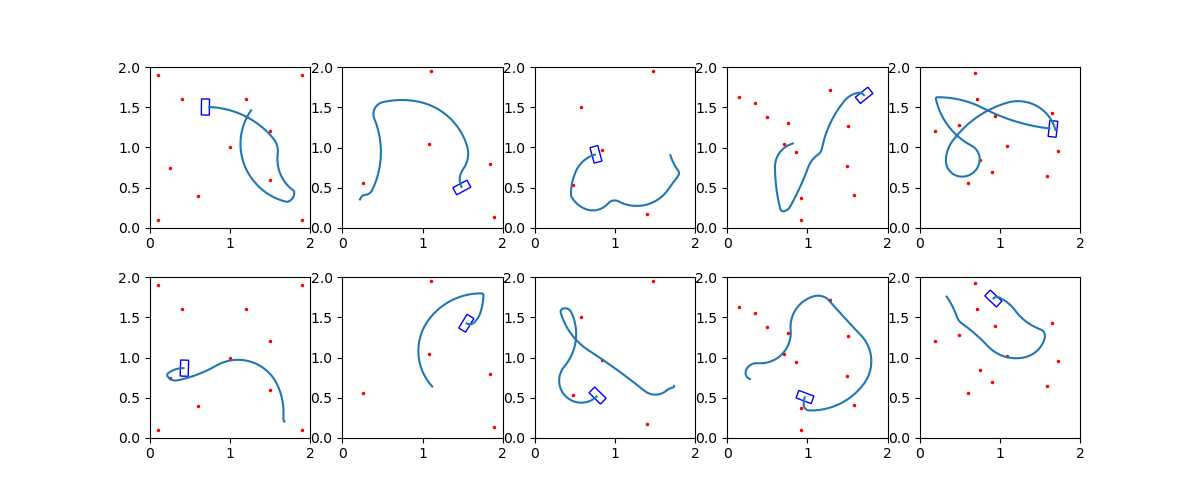
\includegraphics[width=\linewidth]{control_sequences_visualization.png}
Each column corresponds to the landmark maps 0-4 and each row corresponds to a different control sequence 0-1

\section{Integrate Noisy Dynamics and Collect Sensor Readings}
\subsection{Simulate robot's motion and measurements}
\subsubsection{Actuation model}
The ground truth files were generated by integrating forward the controls with added noise, as explained in the assignment 3 pdf. It was ensured that if the control value for either velocity or angular velocity was 0, then the noise added would also be 0. Also, the control values never exceeded the robot's limits, even after noise was added.
\subsubsection{Odometry model}
More Gaussian noise was then added to the executed controls from the previous step. Again, the values were clamped so that they would not exceed the limits of the robot's motor. Also, it was ensured that if the original controls had a value of 0, then the odometer's reading would also be 0.
\subsubsection{Observation model}
The landmark\textunderscore sensor function in simulate.py calculates the distances and angles to each landmark. For distance, the Pythagorean theorem is used. To find the angle in the local robot's coordinates, first, an intermediate angle is found. This angle is equal to the arctan of the ratio between the landmark's rise and the landmark's run in relation to the ground truth configuration. This is done with the arctan2 function provided by numpy. However, we need to account for the robot's heading angle, which is not necessarily 0. So we have to subtract the ground truth angle from this intermediate angle and we get the angle that we want. Finally, the angle is adjusted to be in the range [-pi, pi]. Noise is added to these values from the landmark sensor in accordance with the assignment's instructions.

\subsection{Visualize the dead reckoning solution}
To visualize the dead reckoning solution, FuncAnimation from matplotlib was used. The landmark ground truth positions were drawn and these never change throughout the animation. Each frame, the robot's ground truth position (blue rectangle), odometry position (red rectangle), and landmark observations (red x's) are updated and redrawn. additional blue and red dots are drawn at the ground truth and odometry locations respectively to aid in visualization. Finally, red lines are drawn to connect the odometry motion's current point and each landmark. These lines are updated at each frame. See the dr folder for animations from five selected maps. It is clear that the odometry readings from the high noise files result in motion that strays further from the ground truth path, and as a result the landmark observation locations are more inaccurate too.

\section{Implement Particle Filter for Localization}
\subsection{Given known initial robot pose}

\begin{enumerate}
    \item \textbf{Initialization:} 
    \begin{itemize}
        \item Purpose: To create an initial set of hypotheses (particles) about the state of the system (robot's pose).
        \item Process: Each particle $i$ is initialized with the same state $x_i^0 = \text{initial\_pose}$.
    \end{itemize}
    
    \item \textbf{Prediction:}
    \begin{itemize}
        \item Purpose: To simulate the effect of the motion command on each particle.
        \item Process: For each particle $i$, update its state $x_i$ based on the control input $u$ and motion model, with added noise.
        \item Formula: 
        \[ x_i^{'} = x_i + \begin{bmatrix} v \cdot \cos(\theta) \\ v \cdot \sin(\theta) \\ \omega \end{bmatrix} \cdot dt + \text{noise} \]
        where $v$ and $\omega$ are the linear and angular components of the control input $u$, and $dt$ is the time step.
    \end{itemize}
    
    \item \textbf{Update (Weighting):}
    \begin{itemize}
        \item Purpose: To evaluate each particle's likelihood based on the observed sensor data.
        \item Process: For each particle $i$, compare its predicted state with the actual sensor measurements and update its weight.
        \item Formula:
        \begin{itemize}
            \item For each landmark $j$, calculate the expected measurement $z_{ij}^{exp}$ based on the particle's state.
            \item Compare $z_{ij}^{exp}$ with the actual measurement $z_{ij}^{obs}$.
            \item The weight $w_i$ for each particle is updated based on the likelihood of observing $z_{ij}^{obs}$ given $z_{ij}^{exp}$, which is modeled as a Gaussian distribution:
            \[ w_i = w_i \cdot \prod_j \mathcal{N}(z_{ij}^{obs}; z_{ij}^{exp}, \sigma^2) \]
            \item The likelihood is computed for both distance and angle to each landmark.
            \item Here, $\sigma$ represents the standard deviation of the sensor noise.
        \end{itemize}
    \end{itemize}
    
    \item \textbf{Normalization:}
    \begin{itemize}
        \item Purpose: To ensure the weights sum up to 1.
        \item Formula:
        \[ w_i = \frac{w_i}{\sum_k w_k} \]
    \end{itemize}
    
    \item \textbf{Resampling:}
    \begin{itemize}
        \item Purpose: To focus on particles that are more likely, based on their weights.
        \item Process: Randomly select a new set of particles from the current set, where particles with higher weights are more likely to be selected.
        \item Method: Stochastic universal sampling or similar.
        \item Result: A new set of particles, which will undergo the prediction step in the next iteration.
    \end{itemize}
    
    \item \textbf{Repeat Steps 2-5:}
    \begin{itemize}
        \item For each time step or control input, repeat the prediction, update, normalization, and resampling steps.
    \end{itemize}
\end{enumerate}

In summary, the particle filter iteratively predicts the effect of actions, updates particle weights based on sensor observations, normalizes these weights, and resamples the particles to focus on the most likely states. This process enables the filter to approximate the posterior probability distribution of the system's state.

\section{Evaluation and Experiments}
The file evaluation.py generates animations for the estimations gathered from the particle filter. In the assignment instructions, the code is not run with the readings files as a parameter, so in order to include the landmarks observation locations in the animations, the readings file is used corresponding to the x, y, z from the other parameters. Similar to the dead reckoning animations, the robot's locations are drawn with rectangles and the noisy landmark locations are drawn with lines connecting them to the current configuration. The only difference is that the estimated locations from the particle filter are drawn in black and so are the noisy landmarks. 

To the right of the robot animation, plots with animations displaying the error are shown. In the middle plot, the euclidean distance between the ground truth and estimate is plotted on the y axis, and the time on the x axis. In the right plot, the difference between the ground truth angle and the estimated angle is plotted (in radians) on the y axis, and the corresponding time is plotted on the x axis. It was determined that when there was a high amount of noise in readings, there was more error. However, choosing a higher amount of particles decreased this error. However, choosing a high amount of particles severely lowered the performance of the program. See video1 and video2 folders for visualizations.

\subsection{Given known initial robot pose}

\begin{figure}[ht]
    \centering
    \includegraphics[width=\linewidth]{known_0_0_L_200.png}
    \caption{0, 0, L, 200}
\end{figure}
\begin{figure}[ht]
    \centering
    \includegraphics[width=\linewidth]{known_1_0_H_200.png}
    \caption{1, 0, H, 200}
\end{figure}
\begin{figure}[ht]
    \centering
    \includegraphics[width=\linewidth]{known_2_1_L_1000.png}
    \caption{2, 1, L, 1000}
\end{figure}
\begin{figure}[ht]
    \centering
    \includegraphics[width=\linewidth]{known_3_0_H_500.png}
    \caption{3, 0, H, 500}
\end{figure}
\begin{figure}[ht]
    \centering
    \includegraphics[width=\linewidth]{known_4_0_L_200.png}
    \caption{4, 0, L, 200}
\end{figure}


\end{document}
